% XeLaTeX can use any Mac OS X font. See the setromanfont command below.
% Input to XeLaTeX is full Unicode, so Unicode characters can be typed directly into the source.

% The next lines tell TeXShop to typeset with xelatex, and to open and save the source with Unicode encoding.

%!TEX TS-program = xelatex
%!TEX encoding = UTF-8 Unicode

\documentclass[a4paper,bachelor]{ructhesis}

%自添宏包
\usepackage{skak}%国际象棋
\usepackage{subfigure}%子图http://www.ctex.org/documents/latex/graphics/node111.html
\usepackage{chemfig}%化学式
\usetikzlibrary{trees}



%将封面信息补全,相关专业名称过长的请在文字前添加命令\ziju{-0.15}
%文头
\sign{中国人民大学本科毕业论文}
%\sign{硕士学位论文}
%\sign{博士学位论文}



%以下信息本科研究生都需要补全
\title{中国人民大学LaTeX模板}%论文题名
\author{许白黑}%作者
\school{}%学院
\field{\ }%专业
\studentid{2012202000}%学号
\advisor{}%指导老师
\date{2015年12月11日}


%以下本科填写
\grade{}%年级
\score{4.0}%成绩
\thesiscode{论文编码:RUC-BK-专业代码}%论文编码
\subtitle{}%论文副题名,没有不填写


%以下研究生填写
\etitle{LaTeX template of Renmin university of China}%英文题目
\keywords{\TeX{}}%论文主题词
%摘要关键词
\keywordzh{中文摘要关键词}%中文摘要关键词
\keyworden{English\qquad template}%英文摘要关键词


%
\begin{document}

%扉页
\maketitle

%独创性声明
\originality
%授权书在这插入
\authorization{figures/shouquan.png}
%中文摘要
% the abstract
\begin{abstractzh}
RUCThesis 是根据中国人民大学《本科论文指导手册》和《研究生学位论文及其摘要的撰写和印制要求》而制作的 LATEX 论文模板。
\end{abstractzh}
%英文摘要
% the abstract
\begin{abstracten}
This is an English Abstract.
\end{abstracten}



\frontmatter

%正文目录
\tableofcontents
%插图目录
\listoffigures
%表格目录
\listoftables


\mainmatter\clearpage
\pagestyle{fancy}

%正文章节
\chapter{\LaTeX{} 介绍}
%\section{安装\LaTeX{} }
%\subsection{Mac OS X}
%\begin{figure}[htbp]
%\centering\includegraphics[width=5cm,height=1.32cm]{figures/Logo_2.pdf}
%\caption[示意图]{用LaTeX画图}
%\end{figure}
\LaTeX\footnote{https://zh.wikipedia.org/wiki/LaTeX}(英语发音:/ˈleɪtɛk/ lay-tek或英语发音:/ˈlɑːtɛk/ lah-tek,音译“拉泰赫”),文字形式写作\LaTeX ,是一种基于\TeX\ 的排版系统,由美国电脑学家莱斯利·兰伯特在20世纪80年代初期开发,利用这种格式,即使用户没有排版和程序设计的知识也可以充分发挥由\TeX\ 所提供的强大功能,能在几天,甚至几小时内生成很多具有书籍质量的印刷品。对于生成复杂表格和数学公式,这一点表现得尤为突出。因此它非常适用于生成高印刷质量的科技和数学类文档。这个系统同样适用于生成从简单的信件到完整书籍的所有其他种类的文档。

\LaTeX\ 使用\TeX\ 作为它的格式化引擎,当前的版本是\LaTeX 2ε。
\begin{figure}[htbp]
\centering
\subfigure[国际象棋]{ 
	\label{fig:mini:subfig:a} %% label for first subfigure 
	\begin{minipage}[b]{0.5\textwidth} 
	\centering 
	\fenboard{%
	r5k1/%
	1b1p1ppp/%
	p7/%
	1p1Q4/%
	2p1r3/%
	PP4Pq/%
	BBP2b1P/%
	R4R1K w - - 0 20}
	\mbox{}\showboard
	\end{minipage}}% 
\subfigure[化学式]{
	\label{fig:mini:subfig:b} %% label for second subfigure 
	\begin{minipage}[b]{0.5\textwidth} 
	\centering 
      	\chemfig{
 	H_3C-[:72]{\color{blue}N}*5(- 
	*6(-(={\color{red}O})-
	{\color{blue}N}(-CH_3)-
	(={\color{red}O})-
	{\color{blue}N}(-CH_3)-=)--
	{\color{blue}N}=-)}
   	 \end{minipage}} 
\caption{\LaTeX\ 绘图示例} 
\label{fig:mini:subfig} %% label for entire figure 
\end{figure}


\chapter{\RUCThesis\ 介绍}
\RUCThesis\ 是我在学校本科和研究生规定(虽然大部分时间都在迎合这基于word的规定)的基础上写出来的。\par
\section{必要的宏包}
本模板中包含的宏包如下表所示:
\begin{table}[htb]
  \centering
  \begin{minipage}[t]{0.8\linewidth} 
  \caption[必要宏包]{本模板中包含的宏包,当然这些必须安装。其实这些在你的\LaTeX\ 里面已经有了。其实这还是一个简单三线表的例子,其实这还是一个长表格标题的例子,当然还是一个表格中插脚注的例子。}
  \label{tab:template-files}
    \begin{tabular*}{\linewidth}{cccccc}
      \toprule[1.5pt]
       \multicolumn{6}{c}{\sf 宏包文件}\\ \midrule[1pt] 
      ctexbook & geometry & hyperref & graphicx\footnote{插图宏包} & titletoc & ifxetex \\ 
      ifthen  & calc & lscape\footnote{页面横向放置宏包}   & multicol & color   & pstricks\\
      \bottomrule[1.5pt]
    \end{tabular*}
  \end{minipage}
\end{table}

\section{编译源文件}
如果已经有ructhesis.cls文件的可以直接使用。
目前的版本还没有参考文献样式,先借用了一个(可能会报错)。 
在main.tex文件下使用如下命令:

这里我们使用xelatex作为引擎,第一步为编译main.tex文件,第二步处理参考文献,然后再编译两遍生成pdf文件\\
{\tt
\$ xelatex main.tex\\
\$ bibtex main.tex\\
\$ xelatex main.tex\\
\$ xelatex main.tex\\}
\section{编译模板文件}
想编译模板文件和生成手册的可以执行下述代码\par
生成模板文件{\tt ructhesis.cls}\\
{\tt\$ latex ructhesis.ins}\\
生成手册{\tt ructhesis.pdf\\
\$ xelatex ructhesis.dtx\\
\$ makeindex -s gind.ist -o ructhesis.ind ructhesis.idx\\
\$ makeindex -s gglo.ist -o ructhesis.gls ructhesis.glo\\
\$ xelatex ructhesis.dtx\\
\$ xelatex ructhesis.dtx}
\section{扉页}
\subsection{宏}

在{\tt main.tex}文件里面根据
\begin{landscape}
\begin{figure}[htbp]
\centering
\tikzstyle{every node}=[anchor=west]
\begin{tikzpicture}[%
  grow via three points={one child at (0.5,-0.7) and
  two children at (0.5,-0.7) and (0.5,-1.4)},
  edge from parent path={(\tikzparentnode.south) |- (\tikzchildnode.west)}]
  \node {\RUCThesis\ }
child { node {chap}
    	child { node {chapter1.tex\quad \% 章节文件}}
      	child { node {...}}
      	child { node {appendix\_{}1.tex\quad \% 附录}}} 
child [missing] {} 
child [missing] {} 
child [missing] {}
child { node {cover.tex\quad \% 封面文件}}
child { node {figures}
	child { node {logo.pdf\quad \% 图像}}
	child { node {...}}}
child [missing] {} 
child [missing] {} 
child { node {format}
    	child { node {acknowledge.tex\quad \% 致谢}}
      	child { node {authorization.tex\quad \% 授权书影印件}}
      	child { node {cabstractpage.tex\quad \% 中文摘要}}
	child { node {eabstractpage.tex\quad \% 英文摘要}}
      	child { node {Originality.tex\quad \% 独创性声明}}} 
child [missing] {} 
child [missing] {} 
child [missing] {}
child [missing] {} 
child [missing] {} 
child { node {main.tex\quad \% 主文件}}
child { node {ref}
	child { node {ruc.bst\quad \% 参考文献样式}}
	child { node {yourbib.bib\quad \% 参考文献数据库}}}
child [missing] {} 
child [missing] {} 
child { node {ructhesis.cls\quad \% \RUCThesis\ 文档类}};
\end{tikzpicture}
\caption{\RUCThesis\ 文件目录} 
\end{figure}
\end{landscape}
\section{\RUCThesis\ 文档类}

\section{扉页}
\subsection{宏}
在{\tt main.tex}文件里面根据


\chapter{使用方法}
\section{{\tt main.tex}文件}
将文档类选择{\tt ructhesis},文档的选项有{\tt bachelor、master、promaster、doctor}代表不同的学位论文排版方式。\par 
在导言区填写扉页相关信息和摘要关键词(需要在关键词间按照本科或者研究生的规定输入空格)。\par

\begin{longtable}[c]{ll}
\caption{命令(环境)解释}\label{tab:performance}\\
\toprule[1.5pt]
命令(环境) & 意义\\\midrule[1pt]
\endfirsthead
\caption[]{命令(环境)解释(续)}\\
\toprule[1.5pt]
 命令(环境) & 意义\\\midrule[1pt]
\endhead
\hline
\multicolumn{2}{r}{续下页}
\endfoot
\endlastfoot
{\tt \textbackslash maketitle}  & 插入扉页 \\
{\tt \textbackslash originality}  &  插入独创性声明 \\
{\tt \textbackslash authorization}  & 插入授权书\\
{\tt \textbackslash tableofcontents}  & 正文目录 \\
{\tt \textbackslash listoffigures}  & 插图目录 \\
{\tt \textbackslash listoftables}  & 表格目录 \\
{\tt \textbackslash autograph}  & 本科签名\footnote{插入签名,在普通章节文件中插入无限制,但在\tt main.tex\rm 文件插入时被插入的章节不能使用\tt\textbackslash include\rm 命令,需使用\tt\textbackslash input\rm 命令。}  \\
{\tt \textbackslash appendix}  & 附录 \\
{\tt \textbackslash bibliographystyle}  & 参考文献样式 \\
{\tt \textbackslash bibliography}  &参考文献数据库 \\
{\tt \textbackslash addcontentsline}  & 加入目录 \\
{\tt abstractzh}  & 中文摘要环境 \\
{\tt abstracten}  & 英文摘要环境 \\
{\tt acknowledge}  & 致谢环境 \\
\bottomrule[1.5pt]
\end{longtable}
\section{{\tt cover.tex}文件}
在{\tt cover.tex}文件中,可以有博士:doctor,学硕:master,专硕:promaster,本科:bachelor,这几个选项。还有shuji选项用于输出书脊。其中{\tt \textbackslash cover}命令用来生成封皮。在有shuji选项的时候可以利用{\tt \textbackslash covertitle}命令制定书脊文字。具体的各个封皮的配色方案和样式(无图中虚线)如下图所示:
\begin{figure}[htbp]
\centering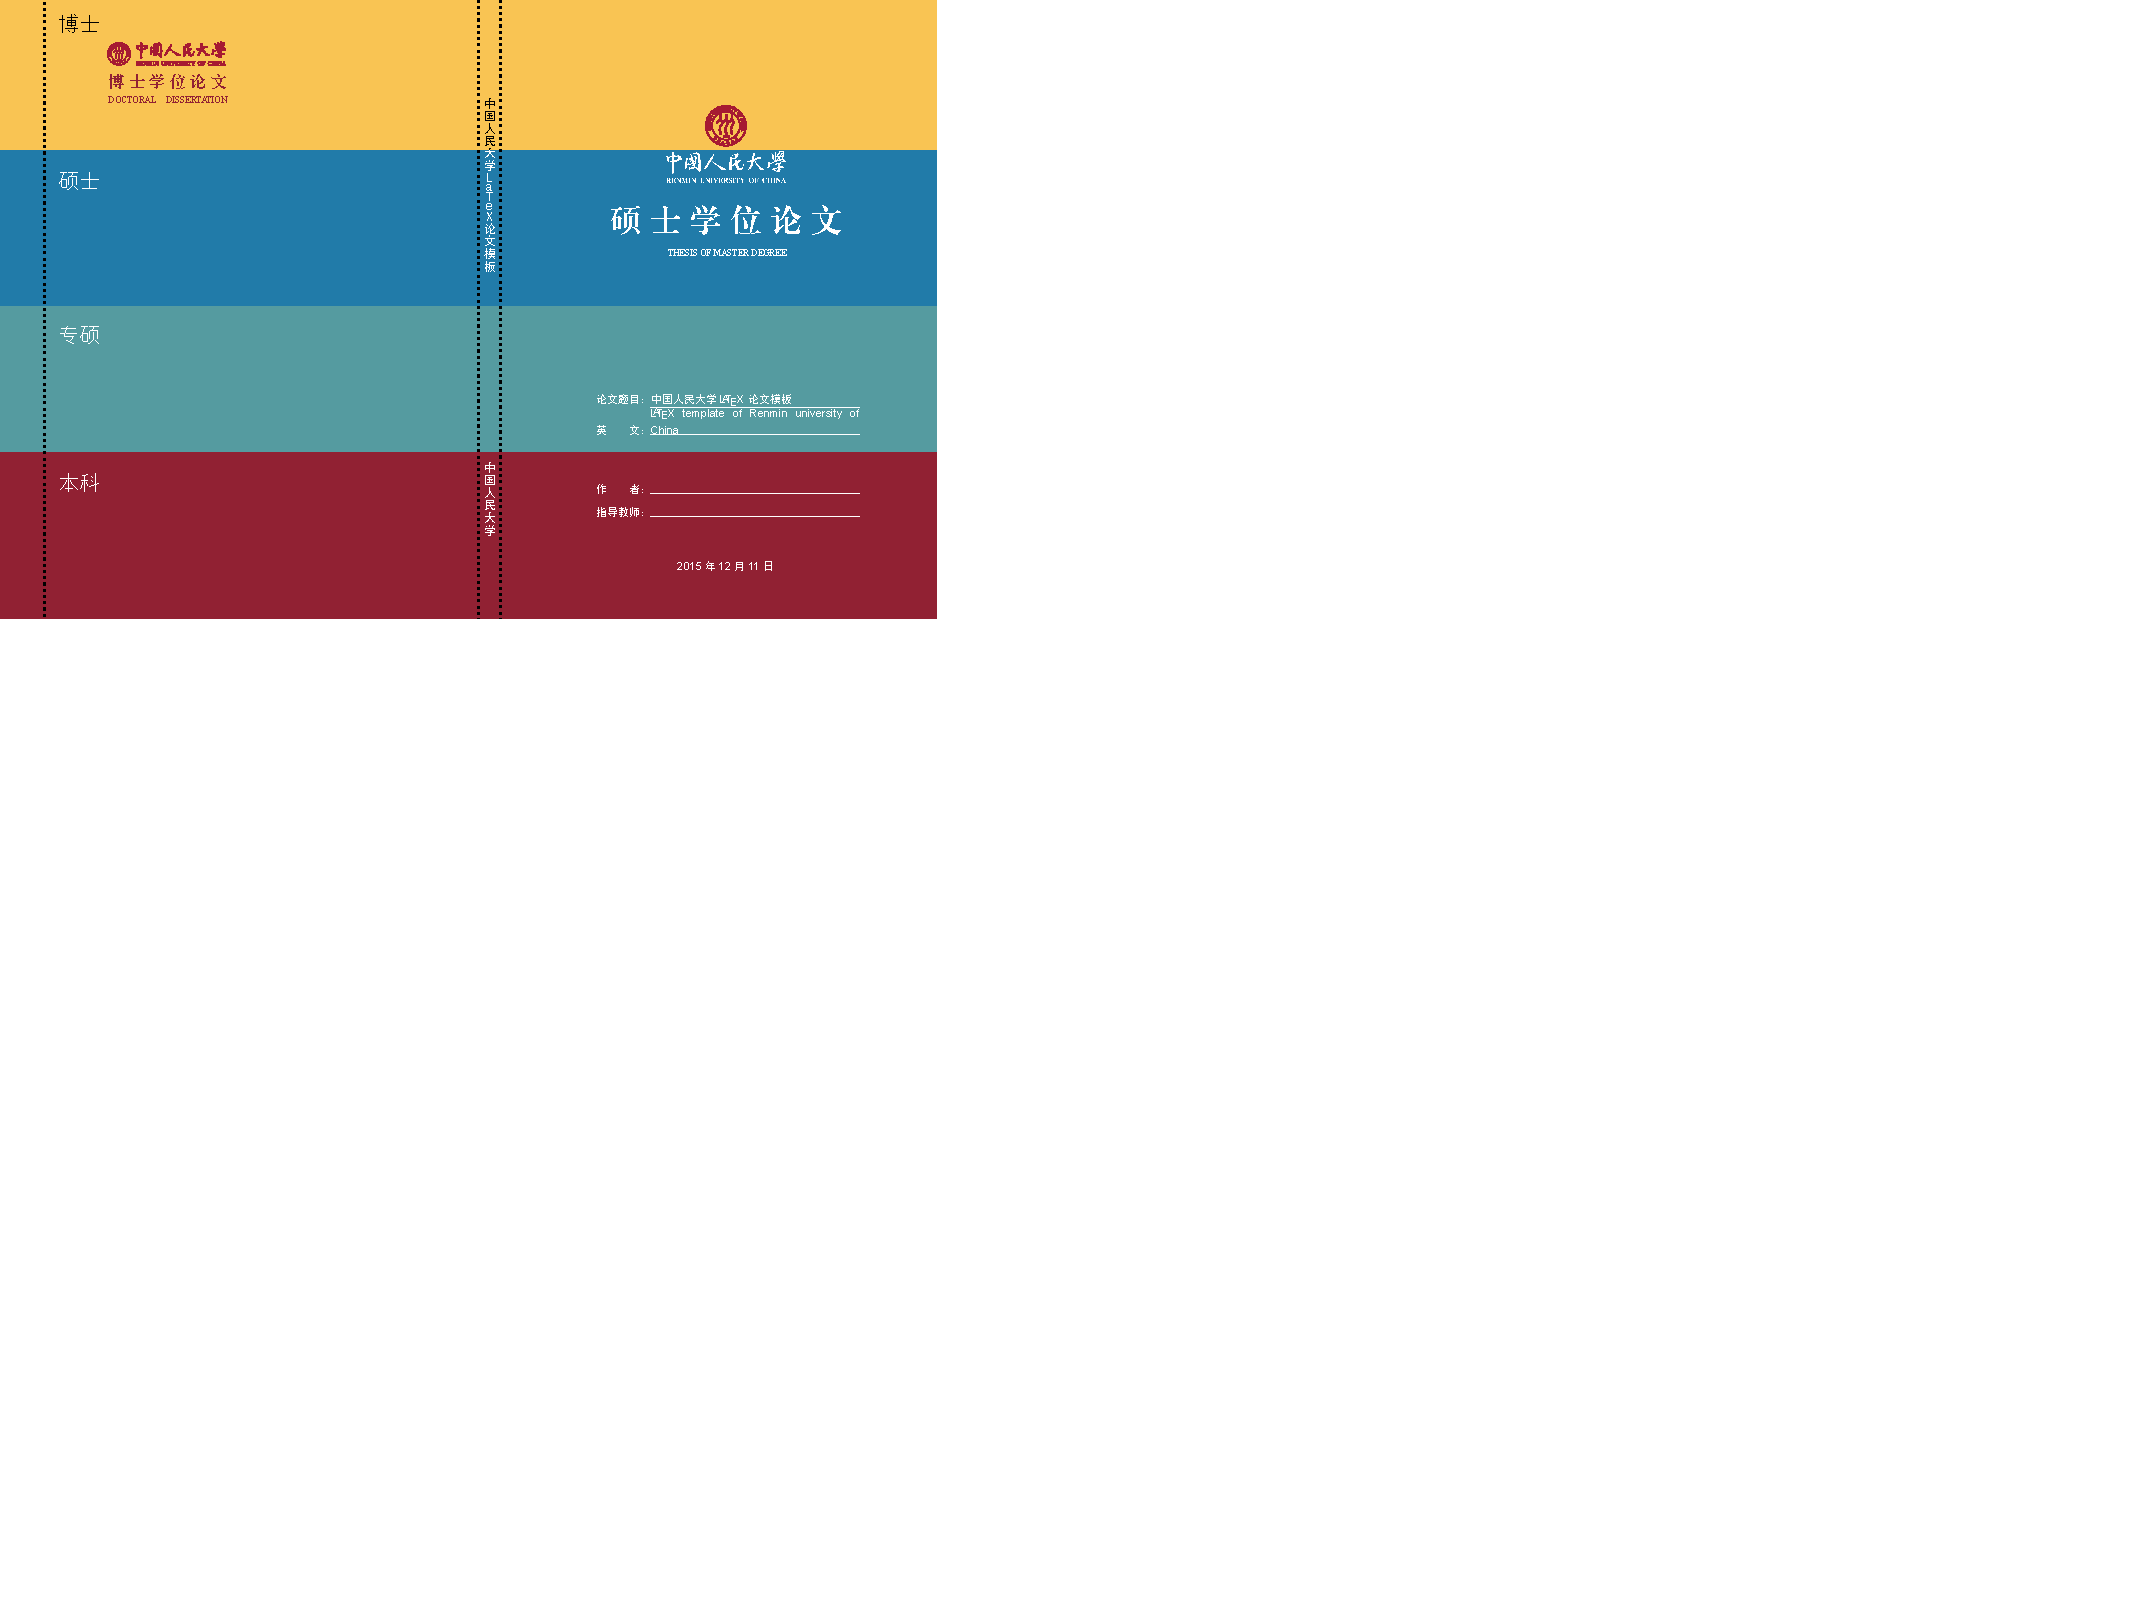
\includegraphics[width=14cm,height=9.24cm]{figures/coverpic.pdf}
\caption[cover示意图]{cover示意图}
\end{figure}
\chapter{一些例子}
\section{各种例子}
\subsection{插图表格}
\begin{figure}[htbp]
\centering
\includegraphics[width=5cm,height=1.32cm]{figures/logo3.pdf}
\caption[中英校名]{中英校名}
\end{figure}
\begin{table}[htbp]
\noindent\begin{minipage}{0.5\textwidth}
\centering
\caption{并排子表格}
\label{tab:parallel1}
\begin{tabular}{p{2cm}p{2cm}}
\toprule[1.5pt]
姓名 & 性别 \\\midrule[1pt]
李狗蛋 & 女 \\\bottomrule[1.5pt]
\end{tabular}
\end{minipage}
\begin{minipage}{0.5\textwidth}
\centering
\caption{并排子表格}
\label{tab:parallel2}
\begin{tabular}{p{2cm}p{2cm}}
\toprule[1.5pt]
姓名 & 性别 \\\midrule[1pt]
张狗蛋 & 女 \\\bottomrule[1.5pt]
\end{tabular}
\end{minipage}
\end{table}
\begin{table}[htbp]
\centering
\caption{并排子表格}
\label{tab:subtable}
\subtable[第一个子表格]
{
\begin{tabular}{p{2cm}p{2cm}}
\toprule[1.5pt]
姓名 & 性别 \\\midrule[1pt]
田狗蛋 & 男 \\\bottomrule[1.5pt]
\end{tabular}
}
\hskip2cm
\subtable[第二个子表格]
{
\begin{tabular}{p{2cm}p{2cm}}
\toprule[1.5pt]
姓名 & 性别 \\\midrule[1pt]
李狗蛋 & 女 \\\bottomrule[1.5pt]
\end{tabular}
}
\end{table}

\subsection{数学环境}
下面是几个数学公式的例子:\par
\begin{equation}
\begin{aligned}
P\{S_n \leq t\} &= \int_{-\infty}^{+\infty}f_{S_n}dt \notag \\
                       &= \int_0^t\frac{\lambda(\lambda u)^{n-1}}{(n-1)!}e^{-\lambda u}du \\
                       &\xlongequal{令 \lambda u=x} \frac{1}{(n-1)!}\int_0^{\lambda t}x^{n-1}e^{-x}dx\\
                       &=\frac{-1}{(n-1)!}(e^{-x}x^{n-1}{\Big|}_0^{\lambda t}-\int_0^{\lambda t}e^{-x}dx^{n-1})\\
                       &=\frac{-1}{(n-1)!}e^{-x}x^{n-1}{\Big|}_0^{\lambda t}+\frac{1}{(n-2)!}\int_0^{\lambda t}e^{-x}x^{n-2}dx
\end{aligned}
\end{equation}\par
再来几个:
\begin{equation}
\begin{aligned}
\lambda &=\left (1+\frac{\left(\frac{\bar{X}-\bar{Y}}{\sqrt{((\frac{1}{n}+\frac{1}{m})\sigma^2)}}\right)^2}{\left(\sqrt{\frac{\sum\limits_{i=1}^n(X_i-\bar{X})^2+\sum\limits_{i=1}^m(Y_i-\bar{Y})^2}{(m+n)\sigma^2}}\right)^2(m+n-2)}\right)^{\frac{n+m}{2}} \\ \notag
            &=\left(1+\frac{T^2}{n+m-2}\right)^{\frac{n+m}{2}}\\
 其中\quad T^2 &=\left(\frac{\frac{\bar{X}-\bar{Y}}{\sqrt{((\frac{1}{n}+\frac{1}{m})\sigma^2)}}}{{\sqrt{\frac{\sum\limits_{i=1}^n(X_i-\bar{X})^2+\sum\limits_{i=1}^m(Y_i-\bar{Y})^2}{(m+n)\sigma^2}}}}\right)^2
\end{aligned}
\end{equation}%要插入本科签名的最后一个章节,插入命令使用\input{}

%本科签名
%\autograph


%参考文献
%\bibliographystyle{ref/rucbib}
%\bibliography{ref/test}
%\nocite{*}
%\addcontentsline{toc}{chapter}{参考文献}

%附录
\appendix
\chapter{如何正确安装\LaTeX\ }

Noun–verb dependencies in various languages and their biological ana- logues. Part A) shows the sentence “Dick saw Jane help Mary draw pictures” trans- lated grammatically into German and Dutch. That is, the words in the sentence are rearranged to reflect the rules of grammar in these two languages, but the sentence is not translated per se. As shown, the English version of the sentence has a rela- tively simple dependency structure between the nouns and verbs that can be modeled using regular grammars. In contrast, German and Dutch require more complicated grammatical models . Part B) shows the biological analogue of the three sen- tences in Part A). Typically, restriction sites can be modeled using regular grammars, whereas complex DNA secondary structures require context–free or context–sensitive grammars . In the first example, the arches are used to represent a “must be followed by” dependency. In the second two examples, they represent a “must be complementary to” dependency.


%致谢
\begin{acknowledge}%致谢
感谢
\end{acknowledge}



\end{document}  






